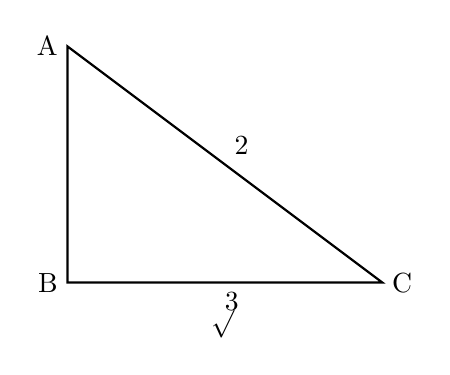
\begin{tikzpicture}[scale=1]

    % Define the vertices of the right-angled triangle
    \coordinate (B) at (0,0);
    \coordinate (C) at (4,0);
    \coordinate (A) at (0,3);

    % Draw the triangle
    \draw[thick] (A) -- (B) -- (C) -- cycle;

    % Add labels for the vertices
    \node[left] at (A) {A};
    \node[left] at (B) {B};
    \node[right] at (C) {C};

    % Add length labels for the sides
    % Length 2 for the hypotenuse AC
    \node[above right] at (2,1.5) {2};
    % \raisebox{-1.5pt} pulls the \surd symbol slightly downwards relative to the 3
    \node[below] at (2,0) {\raisebox{-7.5pt}{$\surd$}$\!\!3$};

\end{tikzpicture}